\chapter{Данные}
В качестве коллекции русскоязычных документов для обучения и тестирования моделей в данной работе используются 4 набора данных. Далее приведено их подробное описание.

\section{Твиты}
Организаторами соревнования Dialogue Evaluate 2016 для дорожки по анализу тональности было предложено 2 набора данных. Оба состояли из сообщений пользователей социальной сети Twitter, так называемые твиты.
Один содержал сообщения, упоминающие банковские компании, а второй был посвящён телекоммуникационным компания.

Особенности:
\begin{itemize}
	\item Размер выборки - около 10 тыс. экземпляров
	\item Максимальная длина документа (сообщения) - 140 символов
	\item Средняя длина документа - 10 слов
	\item Лексикон: сленг, сокращения, эмотиконы
	\item Спец. символы: \# (хэштег), @ (ссылка на пользователя)
	\item Ссылки на внешние ресурсы
\end{itemize}

Таблицы \ref{tab:bank} и \ref{tab:tkk} содержат статистику по числу экземпляров с определенной меткой. Рисунок \ref{fig:hist_twitter} содержит гистограммы с распределением длин документов для данных двух выборок.

\begin{table}[H]
\centering
\caption{Статистика по выборке с банками}
\label{tab:bank}
\begin{tabular}{|c|c|c|c|c|}
\hline
\multirow{2}{*}{Подвыборка} & \multicolumn{4}{c|}{Документы}                \\ \cline{2-5} 
                            & Позитивные & Нейтральные & Негативные & Сумма \\ \hline
Обучающая                   & 760        & 7158        & 2807       & 10725 \\ \hline
Тестовая                    & 318        & 2316        & 784        & 3418  \\ \hline
\end{tabular}
\end{table}

\begin{table}[H]
\centering
\caption{Статистика по выборке с телекоммуникационными компаниями}
\label{tab:tkk}
\begin{tabular}{|c|c|c|c|c|}
\hline
\multirow{2}{*}{Подвыборка} & \multicolumn{4}{c|}{Документы}                \\ \cline{2-5} 
                            & Позитивные & Нейтральные & Негативные & Сумма \\ \hline
Обучающая                   & 1385        & 5213        & 2611       & 9209 \\ \hline
Тестовая                    & 231        & 1062        & 1167        & 2460  \\ \hline
\end{tabular}
\end{table}

\begin{figure}[H]
\caption{Распределение кол-ва слов в документе для выборок с твитами}
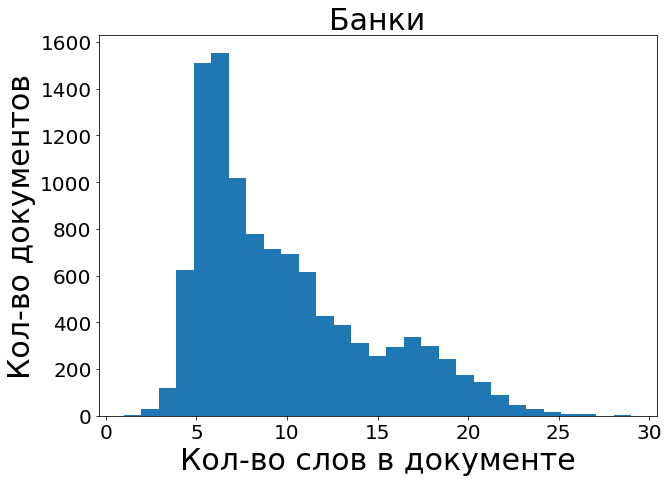
\includegraphics[width=0.5\textwidth]{images/hist_bank.png}
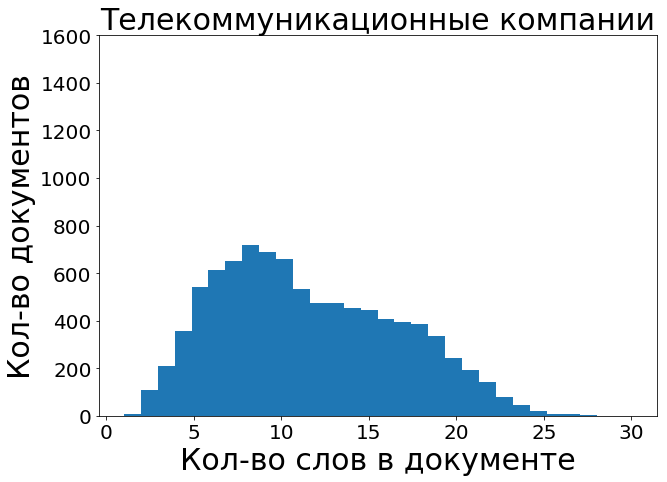
\includegraphics[width=0.5\textwidth]{images/hist_tkk.png}
\label{fig:hist_twitter}
\end{figure}
%--------------------------------------------------------------------------------
\section{Отзывы на товары и рестораны}
Данная выборка содержит отзывы на товары с ресурса \url{www.torg.mail.ru} и отзывы на рестораны с ресурса \url{www.restoclub.ru}.

Особенности:
\begin{itemize}
	\item Размер выборки - около 70 тыс. экземпляров
	\item Максимальная длина документа - 150 слов
	\item Средняя длина документа - 60 слов
\end{itemize}

Таблица \ref{tab:reviews} содержит статистику по числу экземпляров с определенной меткой. Рисунок \ref{fig:hist_reviews} содержит гистограмму с распределением длины документа для данной выборки.

\begin{table}[H]
\centering
\caption{Статистика по выборке с отзывами}
\label{tab:reviews}
\begin{tabular}{|c|c|c|c|}
\hline
\multirow{2}{*}{Подвыборка} & \multicolumn{3}{c|}{Документы}  \\ \cline{2-4} 
                            & Позитивные & Негативные & Сумма \\ \hline
Обучающая                   & 46925        & 12207       & 59132 \\ \hline
Тестовая                    & 11734        & 3050        & 14784  \\ \hline
\end{tabular}
\end{table}

\begin{figure}[H]
\centering
\caption{Распределение кол-ва слов в документе для выборки с отзывами}
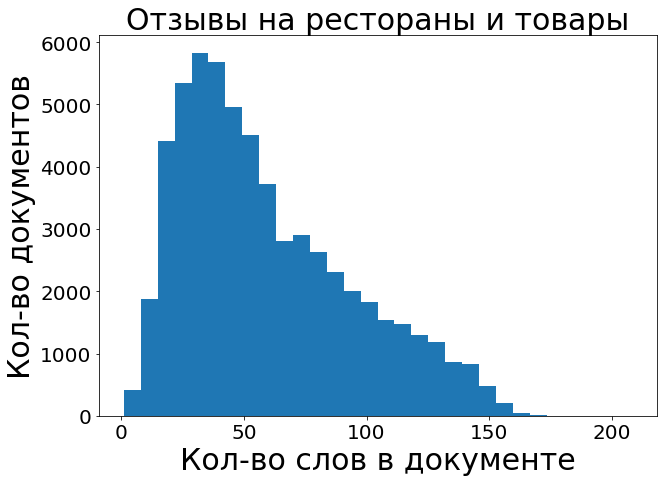
\includegraphics[width=0.5\textwidth]{images/hist_reviews.png}
\label{fig:hist_reviews}
\end{figure}
%--------------------------------------------------------------------------------
\section{Рецензии на фильмы}
Данная выборка содержит рецензии на 350 фильмов с ресурса \url{www.kinopoisk.ru}.

Особенности:
\begin{itemize}
	\item Размер выборки - около 30 тыс. экземпляров
	\item Максимальная длина документа - 1000 слов
	\item Средняя длина документа - 290 слов
\end{itemize}

Таблица \ref{tab:kinopoisk} содержит статистику по числу экземпляров с определенной меткой. Рисунок \ref{fig:hist_kinopoisk} содержит гистограмму с распределением длины документа для данной выборки.

\begin{table}[H]
\centering
\caption{Статистика по выборке с рецензиями}
\label{tab:kinopoisk}
\begin{tabular}{|c|c|c|c|c|}
\hline
\multirow{2}{*}{Подвыборка} & \multicolumn{4}{c|}{Документы}                \\ \cline{2-5} 
                            & Позитивные & Нейтральные & Негативные & Сумма \\ \hline
Обучающая                   & 21695        & 3627        & 3754       & 29076 \\ \hline
Тестовая                    & 5349        & 932        & 989        & 7270  \\ \hline
\end{tabular}
\end{table}

\begin{figure}[H]
\centering
\caption{Распределение кол-ва слов в документе для выборки с рецензиями}
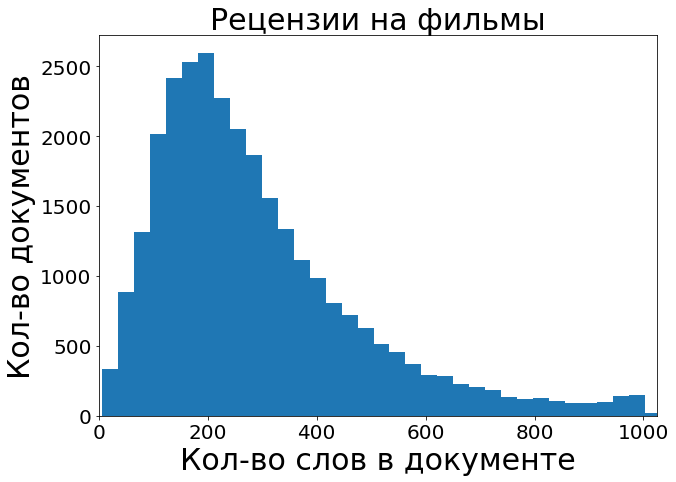
\includegraphics[width=0.5\textwidth]{images/hist_kinopoisk.png}
\label{fig:hist_kinopoisk}
\end{figure}